\subsection{Multi-phase Direct Collocation}\label{s_multiphase}
\noindent Provided the framework to perform a parameter optimization that scales mass and inertial values accordingly, the ollie optimal control problem should be set up next. Section \ref{s_multiphase} will show the method of modeling the ollie phenomena as well as the implementation within the optimization.

\newpage
\subsubsection{General formulation}
\noindent The multi-phase OCP with phases $p \in [1,2,3]$ involves determining the states $\mathbf{q^{(p)}}$, control $u^{(p)}$, phase initial times $t_0^{(p)}$, final times $t_F^{(p)}$, global parameter variables $\sigma$, while maximizing the objective function:
\begin{equation}
    maximize\ \mathcal{J}
\end{equation} 
Subject to the dynamical constraints:
\begin{equation}
\ddot{\mathbf{q}}^{(p)}=\alpha^{(p)}
\end{equation}
with path constraints,
\begin{equation}
        \gamma^{(p)}:\quad \gamma_{min} < ... < \gamma_{max}\\
\end{equation}
and with endpoint constraints:
\begin{equation}
    \beta:\quad \beta_{min} < ... < \beta_{max}
\end{equation}
The ollie OCP will be explained in the order of equations (2-5). Starting with the choice of phases and objective ($\mathcal{J}$). Then describing the dynamic constraints $\alpha$, consisting of the equations of motion (EOM) for the different phases for the human and the skateboard. Followed by the constraints $\gamma$, where the kinetics and kinematics of the human, and friction are implemented. Then endpoint constraints $\beta$, which contain modeling of impact and the bounding of time. The initial and final state and control values are found in Appendix A and are set to a wide margin. If the margin is not set widely, it will be discussed during these paragraphs. All together, this gives all information necessary to solve the ollie OCP. Section \ref{s_summary} gives a summary of the implementations before starting the results section.

In section \ref{s_paropt} are the geometrical variables described that will be optimized. The wheelbase $l_{wb}$, deck length $l_d$, tail length $l_t$, tail inclination $\phi$, truck height $\h_{tr}$, and wheel radius $r_w$ are set as global parameter variables:
\begin{equation}
\begin{array}{rlrl}
    \sigma_{1} &= l_{wb},\ \sigma_{2} &= l_d,\ \sigma_{3} &= l_t,   \\ 
    \sigma_{4} &= \phi,\ \sigma_{5} &= h_{tr},\  \sigma_{6} &= r_w 
\end{array}
\end{equation}

\subsubsection{Phases and Objective} \label{s_phases}
\noindent The phases of the ollie shown in figure \ref{fig:ollie} in section 1 are \cite{frederick_biomechanics_2006}
\begin{itemize}
    \item[(A)]Preparation
    \item[(B)]Pre-pop
    \item[(C)]Pop
    \item[(D)]Upward motion
    \item[(E)]Downward motion
    \item[(F)]Landing
\end{itemize}
For the purpose of the optimization this has been simplified to three phases:
\begin{enumerate} \label{n_phases}
    \item Preparation phase (A,B)
    \item Upward motion (C,D)
    \item Downward motion (E,F)
\end{enumerate}
\noindent I chose to take A and B as one phase, because the dynamics will not change during these phases. Then the same goes for phase C and D, except that compared to phase 1, the dynamics have changed. The skateboard is now airborne, meaning that there is no ground reaction force any more. Furthermore between phases 1 and 2 discontinuities will occur in the velocity states due to impact. By choosing the phase switch at that specific time instance, the discontinuities can be handled during the switch of the phases, creating a continuous domain over both phases. More on this later in section \ref{p_endpoints}. The end of the second phase is chosen such that the objective function can be described properly. Namely, the objective function of the multi-phase optimization needs to be a function of initial or final state variables \cite{brockie_predictive_nodate}. The objective is to ollie as high as possible, thus by choosing the end of phase 2 to be the highest point of the skateboard, the objective can be expressed in terms of final state variables of phase 2. Because a parameter optimization will occur simultaneously with finding the optimal trajectory, the parameters should not be able to influence the objective. For example, if the objective would be to reach maximum height with the tip of the tail, then the parameter optimization will find maximum tail length, tail inclination, truck height, and wheel radius. Because all these variables influence the height of the tip of the tail. To make sure the objective function is independent of the parameter variables, the skateboard is constrained to be level at the highest point and the objective is the middle of a fictional tangent touching lowest point of both wheels. This result in the objective function:

\begin{equation}
    \mathcal{J} = y_s^{(2)}(t_F) + d_{com} - h_{tr} - r_w 
\end{equation}

Where $y_s^{(2)}(t_F)$ is the final state COM location of the skateboard, $d_{com}$ the skateboards' COM to the deck, $h_{tr}$ the truck height, and $r_w$ is the wheel radius.

\subsubsection{System Dynamics}\label{s_systemdynamics}
\begin{figure}
    \centering
    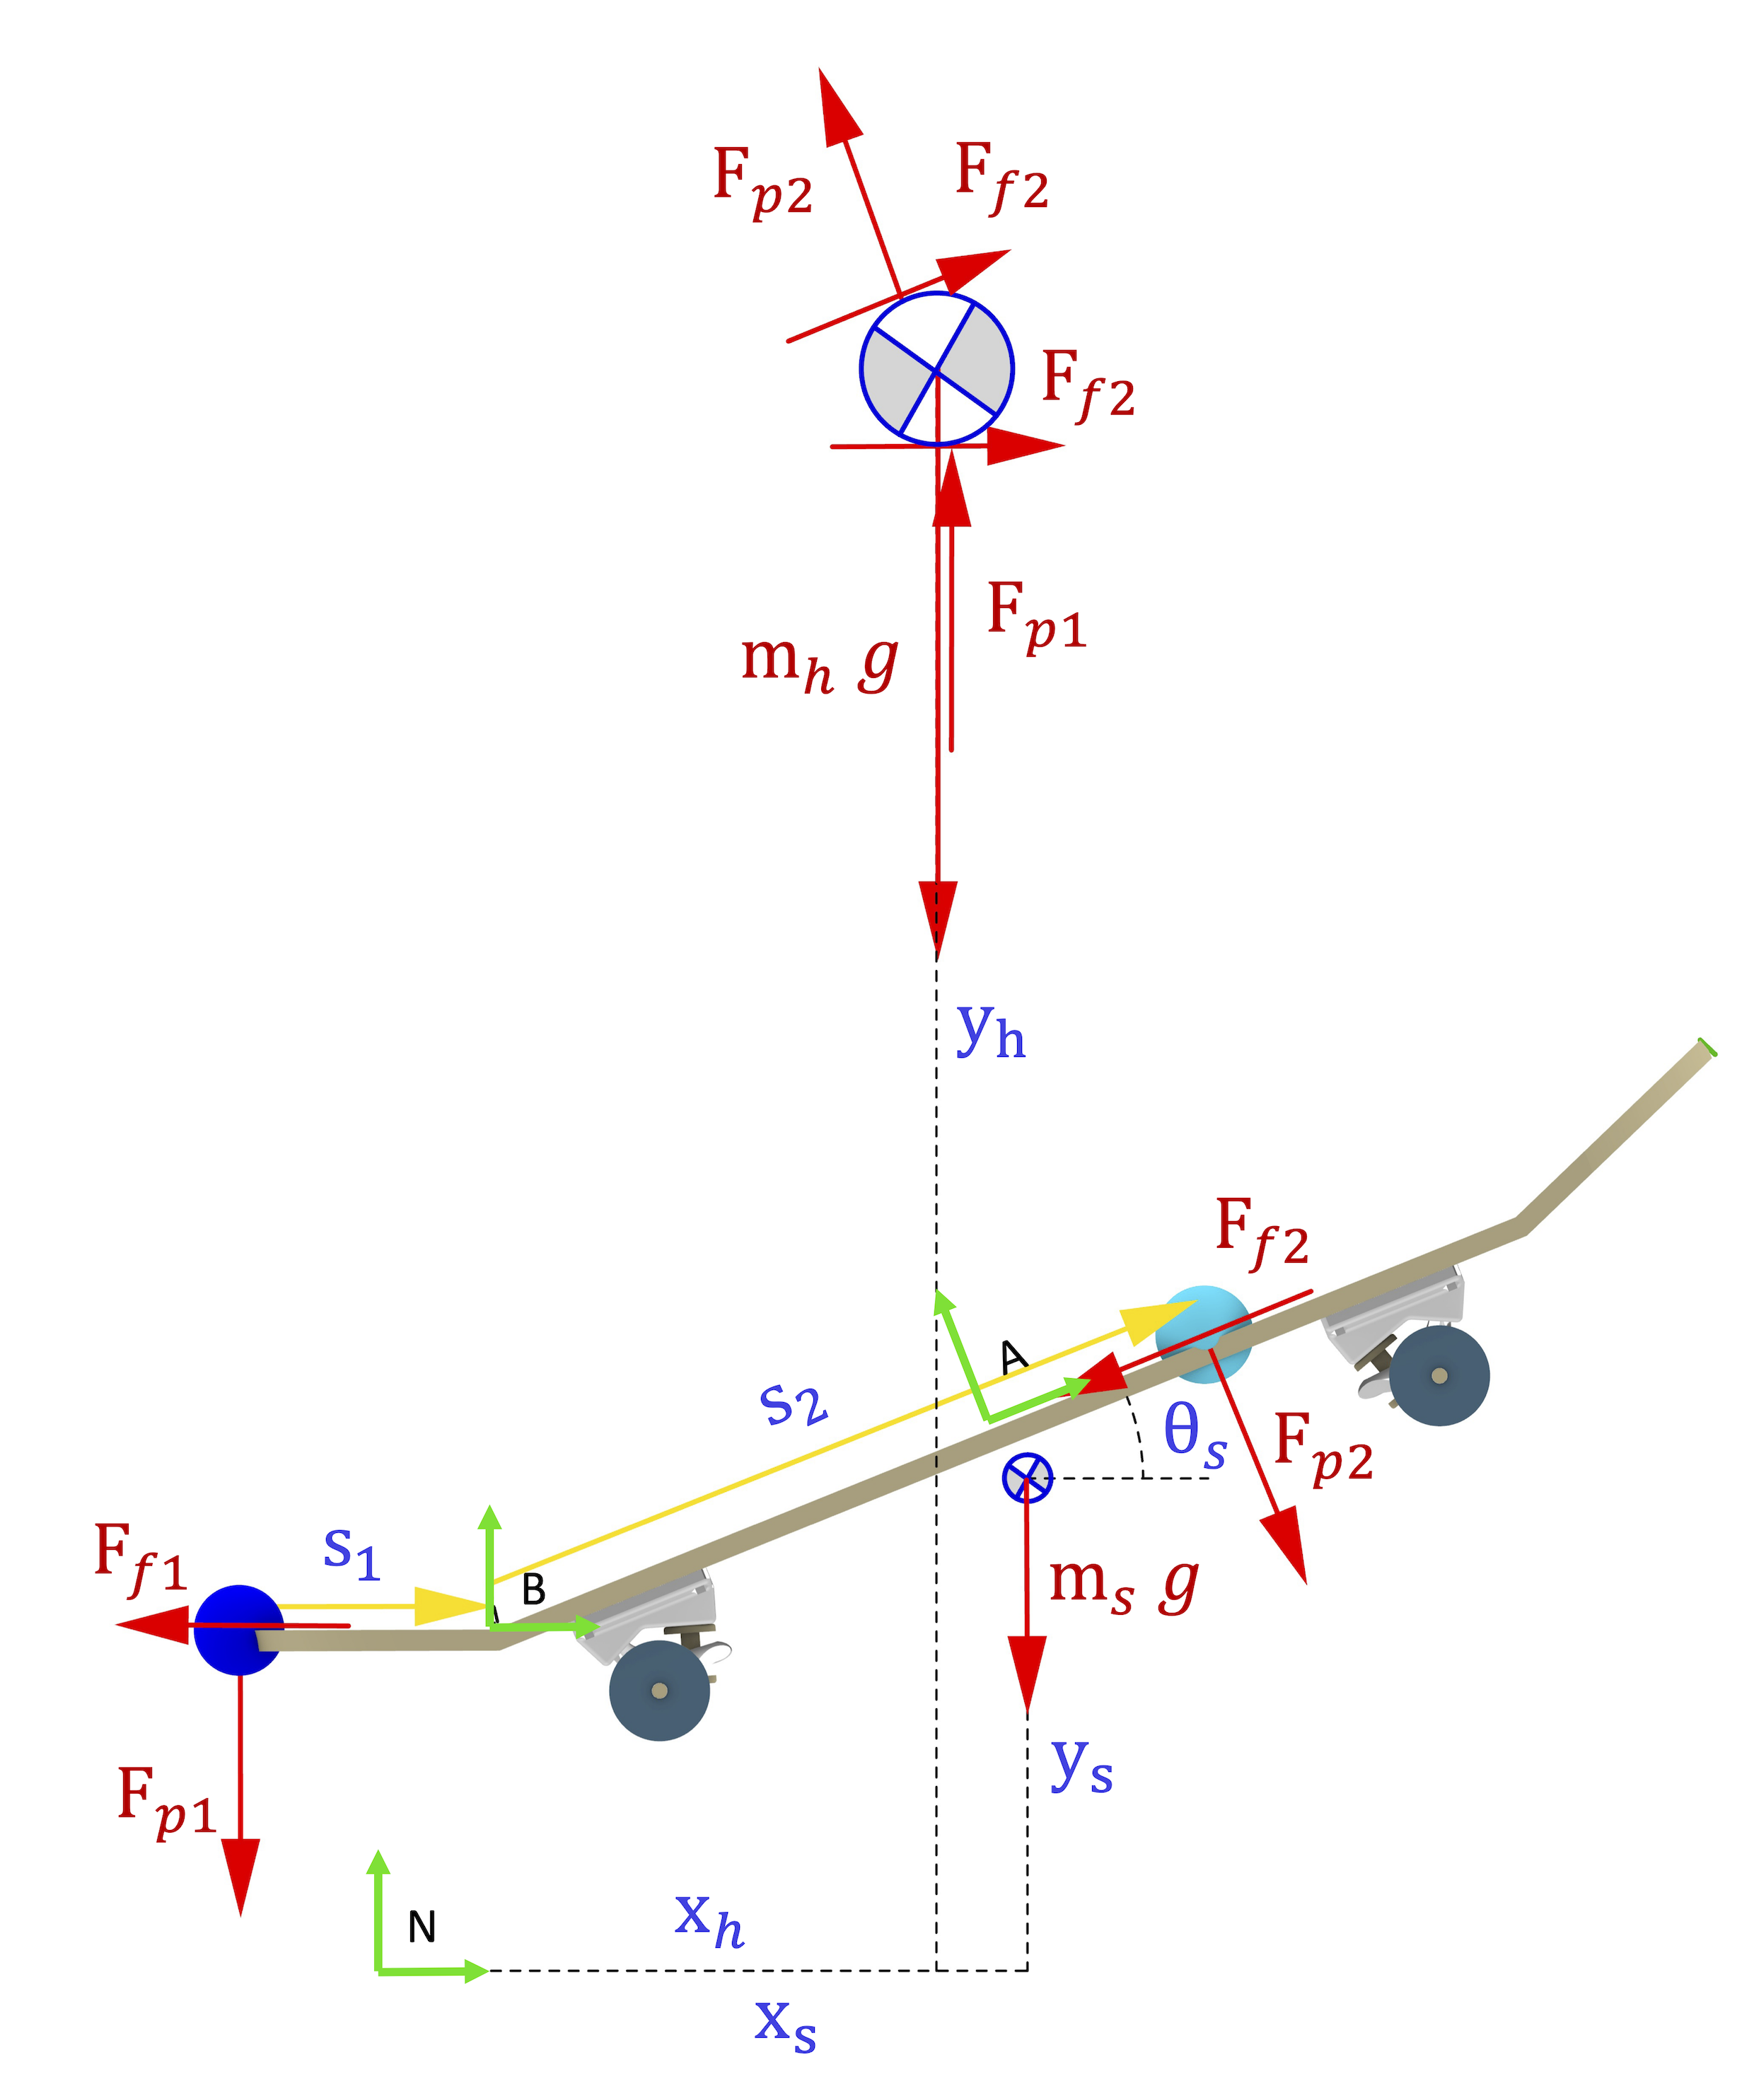
\includegraphics[width=0.45\textwidth]{figure/FBD_skater_feet.png}
    \caption[Free Body Diagrams phase 2 and 3]{Free body diagrams of human and skateboard for phase 1. Blue letters are state variables, Red arrows are forces, the dark blue dot indicates the back foot and the forces that are exerted by the foot. Same goes for the front foot, indicated with a cyan dot. When the foot slides, $s$ is changed and friction will be present. The force exerted by the feet are always perpendicular to the board and can never be negative. Green arrows are frames, N frame is the inertial frame, A and B are body fixed. The forces are equal and opposite acting between the feet and the human centre of mass (top). Skateboard has 3 degrees of freedom, the human has two.}
    \label{f_FBD}
\end{figure}
\noindent The system exists of a point mass (the humans' COM) interacting with a rigid body (skateboard). The interaction between the mass point and the body are simulated with equal and opposite forces acting between the massless feet of the human and the COM of the human. The feet locations can move along the top of the skateboard. In figure \ref{f_FBD} is visible that the forces $F_{p1},F_{p2},F_{f1}$, and $F_{f2}$ are equal and opposite between the feet and the COM. $F_{p1},F_{f2}$ are expressed in the body fixed frame B. $F_{p2},F_{f2}$ are expressed in the body fixed frame A. The perpendicular forces $F_{p1}$, and $F_{p2}$ are positively bound to make sure the feet can never pull perpendicularly on the skateboard. I derived the EOMs using SymPy mechanics and the symbolic toolbox \cite{meurer_sympy_2017}.

\paragraph{Human Equations of Motion}
\noindent I modeled the human as a point mass. The point mass is the COM of a human. The simplification ignores many body segments. Which means this model is not representable in terms of metabolic leg power. Only the mechanical power output can be estimated with this model \cite{van_der_kruk_power_2018}. This is confirmed by Morin in \cite{morin_biomechanics_2018}. With this approximation, inertia of the humans' body and segments is neglected. This is reasonable because during the ollie, the human rotates minimally on top of the skateboard (see figure \ref{f_olliesteps}). The human interacts with the skateboard with forces perpendicular to the skateboard $F_{p1,2}$ and frictional forces tangent to the deck surface ($F_{f1,2}$). These forces are equal and opposite forces between the skateboard and the human as shown in \ref{f_FBD}. The location of these force points are dependent on the location of the feet. The back and front feet are indicated with a blue and cyan dot and are defined on the skateboard with variables $s_1$ and $s_2$ respectively. The kinetics and kinematics of the human will be discussed in the constraint section. The human has two degrees of freedom; $x_h$, and $y_h$. Since the forces on the skateboard are equal and opposite to the human, the EOM are formed from equation \ref{e_Fi} without rotational component and equation \ref{e_newtoneuler} with a different mass matrix $\mathbf{M_h} = [m_h, m_h]^T$ :
The EOMs of the human are found with the Newton Euler equations:
\begin{equation}\label{e_newtoneuler}
\begin{array}{c}
        m_s \cdot \ddot x_s = \sum F_x  \\
        m_s \cdot \ddot y_s = \sum F_y  \\
        I_s \cdot \ddot \theta_s = \sum M_c
    \end{array}
\end{equation}
The forces are expressed in the body fixed frames A, and B. This results in the force of the back foot, force of the front foot and combined the total force acting on the human:
\begin{equation} \label{e_humanforce}
\begin{array}{cc}
      \mathbf{F_{bf}} = F_{p1} \cdot \mathbf{\hat b_y} + F_{f1} \cdot \mathbf{\hat b_x}\\
      \mathbf{F_{ff}} = F_{p2} \cdot \mathbf{\hat a_y} + F_{f2} \cdot \mathbf{\hat a_x}\\
      \mathbf{F_h}    = \mathbf{F_{bf}} + \mathbf{F_{ff}}
\end{array}
\end{equation}
Combining equation \ref{e_newtoneuler} and \ref{e_humanforce} expressed in the inertial frame N gives the EOM for the human for all three phases:
\begin{equation}
    \left[\begin{array}{cc}
        m_h & 0 \\
        0 & m_h \\
    \end{array}\right] \cdot \left[\begin{array}{c}
         \ddot x_h  \\
         \ddot y_h \\
    \end{array}\right]=\left[\begin{array}{c}
        \mathbf{F_h}\cdot \mathbf{\hat n_x}  \\
        \mathbf{F_h}\cdot \mathbf{\hat n_y}\\
    \end{array}\right]
\end{equation}
Which lead to the first two dynamic constraints for all three phases:
\begin{equation}
\begin{split}
        \alpha_{1}^{(1,2,3)} = \frac{\mathbf{F_h}\cdot \mathbf{\hat n_x}}{m_h}\\
        \alpha_{2}^{(1,2,3)} = \frac{\mathbf{F_h}\cdot \mathbf{\hat n_y}}{m_h}
\end{split}
\end{equation}

\paragraph{Skateboard Equations of Motion - phase 1}
\begin{figure}[b]
    \centering
    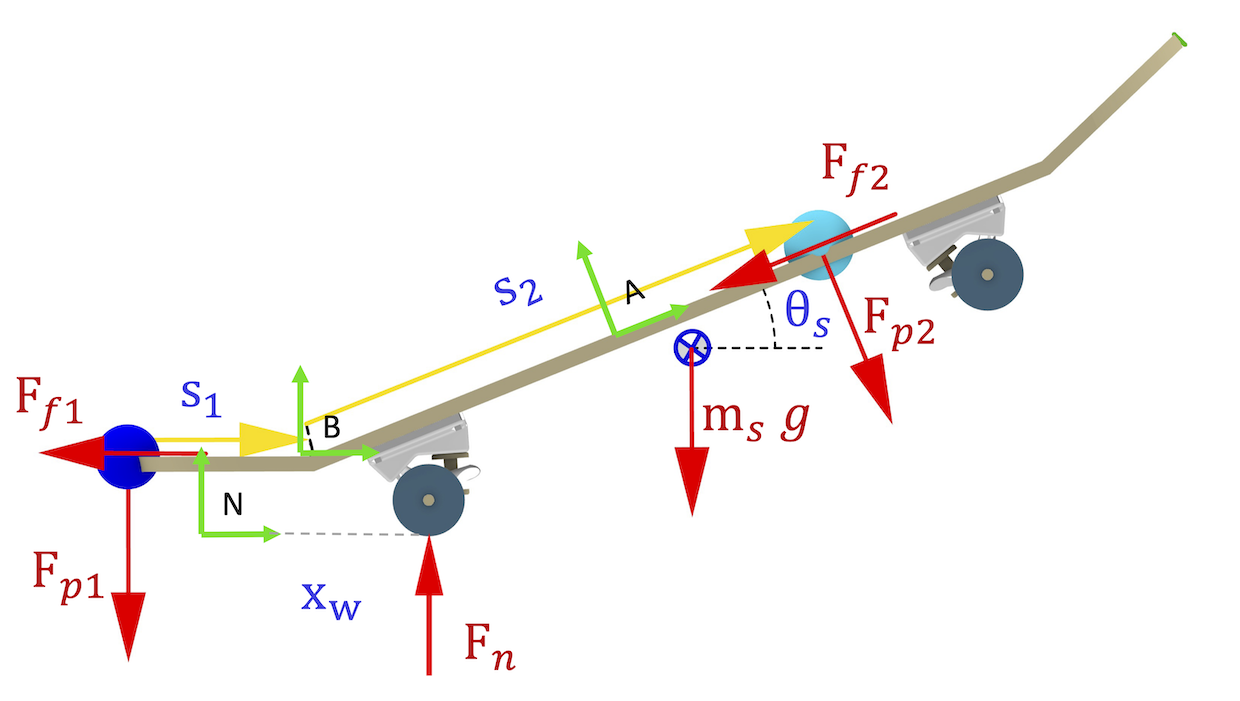
\includegraphics[width = 0.5\textwidth]{figure/FBD_phase1.png}
    \caption[Free body diagram phase 1]{Free body diagram phase 1. The back wheel is now modeled as sliding joint which reduces the degrees of freedom to 2. This is really  similar to the cart-pole problem. The equations are correct as long as the normal force at the wheel is not negative.}
    \label{f_FBDphas1}
\end{figure}
The EOM of the skateboard are derived with the TMT method \cite{vallery_heike_advanced_2018}. As stated in section \ref{s_phases}, the dynamics of phase 1 and 2 are different. The dynamics of phase 2 and 3 are the same. During phase 1 the EOM are derived with a sliding joint at the back wheel. This is done to eliminate the ground reaction forces from the EOM. The COM coordinates are

\begin{equation}
    \mathbf{x} = [x_s, y_s, \theta_s]^T
\end{equation}
The skateboard when considering the back wheel as a joint can be described by two generalized coordinates $x_w$ (x-location back wheels), and $\theta_s$ (angle w.r.t. ground) as shown in figure \ref{f_FBDphas1}. This is done to eliminate the ground reaction forces. The generalized coordinates are:
\begin{equation}
    \mathbf{q} = [x_w, \theta_s]^T
\end{equation}
And the CoM coordinates expressed in the generalized coordinates are:
\begin{equation}
\mathbf{x}=\left[\begin{array}{c}
\frac{l_{w b} \cos \left(\theta_s\right)}{2}+x_w+\left(d_{c o m}-h_{t r}\right) \sin \left(\theta_s\right) \\
\frac{l_{w b} \sin \left(\theta_s\right)}{2}+r_w+\left(h_{t r}-d_{c o m}\right) \cos \left(\theta_s\right) \\
\theta_s
\end{array}\right]
\end{equation}
Differentiating $\mathbf{x}$ once and taking the Jacobian with respect to the velocities gives transformation matrix T:
\begin{equation}
    J_{\dot{\mathbf{x}}}(\mathbf{q}) = \textbf{T} = \left[\begin{array}{c c}
1 & -\frac{l_{w b} \sin \left(\theta_s\right)}{2}+\left(d_{c o m}-h_{t r}\right) \cos \left(\theta_s\right) \\
0 & \frac{l_{w b} \cos \left(\theta_s\right)}{2}+\left(d_{c o m}-h_{t r}\right) \sin \left(\theta_s\right) \\
0 & 1
\end{array}\right]
\end{equation}
Convective terms $\mathbf{g_k}$ are found by taking the Jacobian of $\mathbf{\dot  x}$ with respect to $\mathbf{q}$ and multiplying it by $\mathbf{\dot  q}$ (e.g. $J_{\mathbf{\dot  x}}(\mathbf{q})\cdot \mathbf{\dot  q}$):

\begin{equation}
\mathbf{g_k} = 
\left[\begin{array}{c}
\dot \theta_s^2\left(-\frac{l_{w b} \cos \left(\theta_s\right)}{2}-\left(d_{c o m}-h_{t r}\right) \sin \left(\theta_s\right)\right) \\
\dot \theta_s^2\left(-\frac{l_{w b} \sin \left(\theta_s\right)}{2}+\left(d_{c o m}-h_{t r}\right) \cos \left(\theta_s\right)\right) \\
0
\end{array}\right]
\end{equation}
Two sets of bound vectors are equivalent when they equal resultants and equal moments about any point \cite{moore_force_nodate}. This means that all the forces acting on the skateboard can be described by resultant forces on and moments to the COM. The moments caused by the back and front foot about the COM are $Mc_{bf}, Mc_{ff}$ respectively. Thus the CoM-applied forces and torques $\mathbf{F_{a}}$ are:
 
\footnotesize
\begin{equation}\label{e_Fi}
\begin{array}{c}
    \mathbf{F_{a}}= \left[\begin{array}{c}
-F_{p 1} \sin \left(\phi-\theta_s\right)+F_{p 2} \sin \left(\theta_s\right)-F_{w 1} \cos \left(\phi-\theta_s\right)-F_{w 2} \cos \left(\theta_s\right) \\
-F_{p 1} \cos \left(\phi-\theta_s\right)-F_{p 2} \cos \left(\theta_s\right)+F_{w 1} \sin \left(\phi-\theta_s\right)-F_{w 2} \sin \left(\theta_s\right)-g m_s \\
Mc_{bf} + Mc_{ff}
\end{array}\right] 
\\ \\
Mc_{bf} = -F_{p 1} (-d_{\text {com }} \sin (\phi)-\frac{l_d \cos (\phi)}{2}-l_t+s_1)+F_{w 1}(d_{c o m} \cos (\phi)-\frac{l_d \sin (\phi)}{2})
\\ \\
\footnotesize Mc_{ff} = -F_{p 2}\left(-\frac{l_d}{2}+\mathrm{s}_2(t)\right)+F_{w 2} d_{c o m}
\end{array}
\end{equation}  
\smallskip
\normalsize
The skateboards' mass matrix $\mathbf{M_s} = diag(m_s,m_s,I_s)$ together with the transformed CoM applied coordinates form the EOM of phase 1:
\begin{equation} \label{e_eoma}
    \mathbf{T}^T \mathbf{M_s} \mathbf{T} \cdot \left[\begin{array}{c}
         \ddot x_w  \\
         \ddot \theta_s 
    \end{array}\right] = \mathbf{T}^T (\mathbf{F_a} - \mathbf{M_s} \cdot \mathbf{g_k})
\end{equation}
Rewriting the EoM gives two dynamical constraints valid for phase 1:
\begin{equation}
    \alpha_{3,4}^{(1)} =   \left(\mathbf{T}^T \mathbf{M_s} \mathbf{T} \cdot  \mathbf{T}^T\right)^{-1} (\mathbf{F_a} - \mathbf{M_s} \cdot \mathbf{g_k})
\end{equation}

\paragraph{Flight Equations of Motion - phases 2 and 3}
\noindent The EOM for phases 2 and 3 for the skateboard are without ground contact. The EOMs are derived similarly as the ground EOM, but now there generalized coordinates are the COM coordinates, since the body has 3 degrees of freedom. Thus $\mathbf{q} = \mathbf{x}$, which results in: $J_{\mathbf{\dot x}} \left(\mathbf{q}\right) = diag(1,1,1)$, and $\mathbf{g_k} = [0, 0, 0]^T$.  The COM applied forces $\mathbf{F_a}$ are the same as the ground EOM and don't need to be transformed. This gives the EOM of phases 2 and 3:
\begin{equation}\label{e_eomb}
\mathbf{M_s} \cdot \left[\begin{array}{c}
         \ddot x_s  \\
         \ddot y_s \\
         \ddot \theta_s 
    \end{array}\right] =  \mathbf{F_a}
\end{equation}
Which are in the same form as the Newton Euler equations (eq. \ref{e_newtoneuler}). This leads to the last two dynamic constraints valid for phase 2, and 3:
\begin{equation}
    \alpha_{5,6}^{(2,3)} = (\mathbf{M_s})^{-1}\mathbf{F_a}
\end{equation}
%%%%%%%%%%%%%%%% begin figure %%%%%%%%%%%%%%%%%%%
\begin{figure}[b]%
    \centering
    \subfloat[\centering 45.5" world record ollie. $^{1}$  ]{{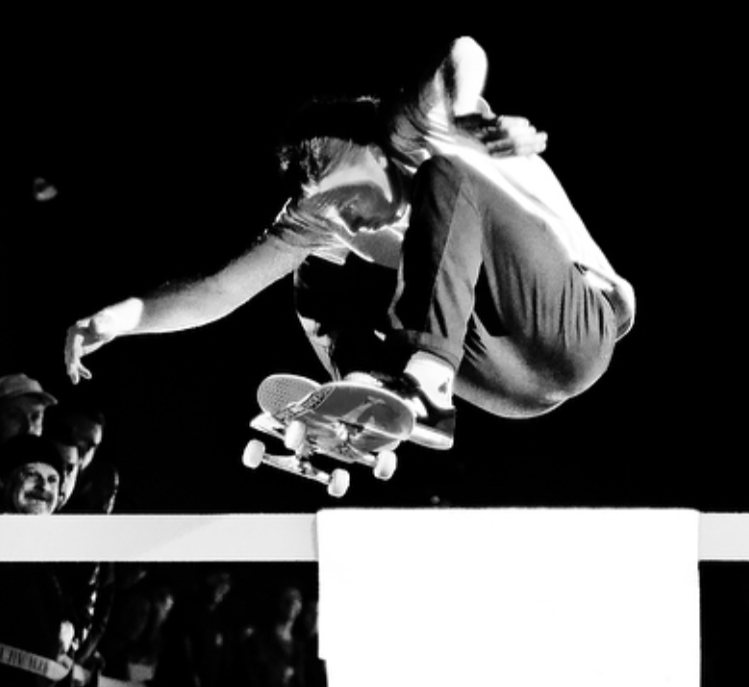
\includegraphics[width=0.2\textwidth]{figure/JakeHayes.png} }}%
    \quad
    \subfloat[\centering Yeadon model in same configuration]{{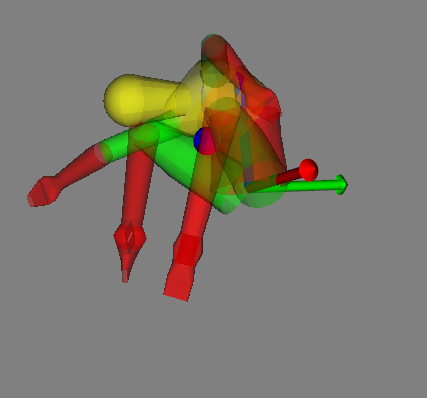
\includegraphics[width=0.2\textwidth]{figure/JakeHayesYeadon.png} }}%
    \caption{Reconstruction of world record ollie} 
    \label{fig:f_record}
    \centering \footnotesize \url{https://theberrics.com/world-record-ollie-footage}$^{1}$%
\end{figure}
%%%%%%%%%%%%%%%% end figure %%%%%%%%%%%%%%%%%%%
\subsubsection{Constraints}
\noindent Now that the dynamics are presented, we can move on to the constraints section. In this section the human kinetics and kinematics will be explained together with the friction model. 

\paragraph{Human}
\noindent The human is simplified as a point mass which reduces complexity for the optimization but sacrifices the reality. To make sure the human as a point mass still gives the output of a more complex model, the kinetics and kinematics will be constrained. 
\subparagraph{Kinematics}
\noindent The kinematics of the human controller are bound by the musculoskeletal restrictions of the human body. The musculoskeletal restricions are difficult to comprise in a point mass model. The first restriction is that the feet can only be within a certain distance of the human COM. This is not simply the leg length, because the COM location of the human will change when the legs are moved. The maximum and minimum feet location with respect to the COM of the human are found with Yeadon, a package for Python to configure a humanoid to a position and find distances between points \cite{yeadon_simulation_1990}. The model is set to a 1.80[m] tall human and is matched to a picture of the world record ollie of Jake Hayes. The reconstruction is seen in fig.\ref{fig:f_record}. The largest possible distance measured with the same model but now configured to an upright position. This leads to the first two constraint:


\begin{equation}\label{\e_yeadon}
\begin{split}
    \gamma_{1}^{(2,3)}:\quad  0.466 < y_h - \mathbf{r_{comH \mathbin{/} bf}} \cdot \mathbf{\hat n_y} < 1.13 \\ 
    \gamma_{2}^{(2,3)}:\quad  0.466 < y_h - \mathbf{r_{comH \mathbin{/} ff}} \cdot \mathbf{\hat n_y} < 1.13 
\end{split}
\end{equation}
These constraints describe that the vertical ($\mathbf{ \hat n_y}$) distance between the feet and the COM can never be outside of the given bounds. The constraint will become very complex if it would be the magnitude of the vector between the feet and the COM thus a vertical approximation is chosen. This constraint will not exceed musculoskeletal limits if the feet do not separate an an extreme distance (split). To make sure this behaviour does not happen, another constraint is implemented that the feet should never be separated more from each other than within a reasonable operating distance.
\begin{equation}
        \gamma_{3}^{(1,2,3)}:\quad   0.1 < |\mathbf{r_{bf/ff}}| < 1
\end{equation}
The skater should not leave the board in horizontal direction either. This gives the next constraint:
\begin{equation}
    \gamma_4^{(1,2,3)}:\quad  -0.3 < x_h - \mathbf{r_{comS\mathbin{/}comH}}\cdot \mathbf{\hat n_x} < 0.3
\end{equation}

To make sure the feet never leave the skateboard, $s_1$ and $s_2$ are positively bound from the end of the tail and the left pocket of the deck respectively (see fig \ref{f_FBD}. To make sure the feet do not leave the skateboard on the other end of the parts, two constraints are added:
\begin{equation}
\begin{array}{c}
    \gamma_{5}^{(1,2,3)}:\quad  0 < s_1-l_t < \infty  \\
    \gamma_{6}^{(1,2,3)}:\quad  0 < s_2-l_d < \infty  \\
\end{array}
\end{equation}
The feet can still be in a no contact scenario as seen in section \ref{ss_mechanics}. This is simulated by when zero force is exerted. 

\subparagraph{Kinetics}
\noindent The kinetics of the human are bound to the characteristics of the countermovement jump (CMJ) during the first phase of the ollie. The CMJ motion is chosen because, 76.3\% of the variance in the performance of the ollie maneuver can be explained by the CMJ (CMJ) \cite{candotti_lower_2012}. The CMJ is reported to have good reliability and is a strong assessment of lower-body mechanical power \cite{barker_relationships_2018}. During a vertical jump, joint torques, knee extensor force, hip abduction forces all map to one output variable: the ground reaction force. The only sensible way to capture the kinetics of a human jumper for a point mass model is the ground reaction force, because only more complex approximation can capture contributions of individual segments. Thus, the ground reaction force of the CMJ is used to realize a realistic COM human jumper model. In figure \ref{f_cmj} a typical ground reaction force for a CMJ is shown. By constraining the vertical rate of force development (RFD) ($dF/dt$, slope in figure \ref{f_cmj}), the maximum force $F_{max}$, maximum displacement $\Delta s$, and maximum mechanical power $P$, the total mechanical output of the legs is constrained for a simple point mass model. By constraining the RFD, the shortening or lengthening cycle is simulated. The maximum force will make sure the force does not exceed the maximum capabilities. By constraining the power, given a constrained force, the maximum velocity is also constrained due to $P = F v_{rel}$.
Due to a constrained maximum distance($\Delta s$) the force can work over, the work done is also constrained due to $W = F ds$, given a constrained force. The data for the RFD, $F_{max}$, $\Delta s$, $P$ is taken from a Division-I male, soccer players with a mean height of 179.5[cm], weight of 75.5[kg], and age of 19.65 years \cite{barker_relationships_2018}. $\Delta s$ and $P$ are calculated in the paper with a point mass approximation which is important to map to the optimization properly. The data was measured for two legs simultaneously, which is unfortunate for the optimization since the two legs can work separately and which might lead to different kinetic data. Though, the constraints are set on the sum of the forces and the forces separately due to the possibility of out of phase pushing and pulling which could result in a combined satisfaction of the constraint but individual legs could exceed the physical limitations. The maximum distance is constraint implemented similar to equation \ref{\e_yeadon} with the same upper bound:
\vspace{-0.1in}
\begin{equation}
\begin{split}
        \gamma_{7}^{(2,3)}:& \quad  1.13-\Delta s < y_h - \mathbf{r_{comH \mathbin{/} bf}} \cdot \mathbf{\hat n_y} < 1.13 \\ 
      \gamma_{8}^{(2,3)}:& \quad  1.13-\Delta s < y_h - \mathbf{r_{comH \mathbin{/} ff}} \cdot \mathbf{\hat n_y} < 1.13 
      \end{split}
\end{equation}

\begin{figure}
    \centering
    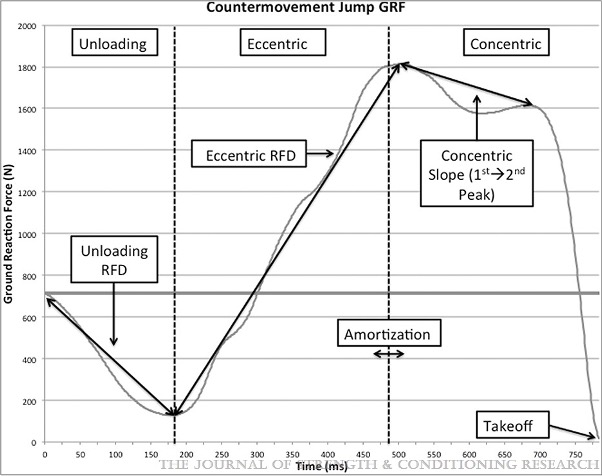
\includegraphics[width=0.4\textwidth]{figure/countermovementjumpRFD.jpg}
    \caption[Ground reaction force of CMJ]{Phases during CMJ. During unloading, the human lowers their COM quickly. During the eccentric phase, the gained downward velocity during the unloading phase is braked until the lowest point is reached which is at the amortization. During the concentric phase the legs are stretched out and upward speed is gained until the take-off. At take-off the vertical speed is maximal.}
    \centering \footnotesize Source: \cite{barker_relationships_2018}%
    \label{f_cmj}
\end{figure}
\noindent The maximum force constraints are set at the sum of all vertical forces $\mathbf{F_h}\cdot \mathbf{\hat n_y}$, and to the vertical components of the back and front feet ($\mathbf{F_{bf}}\cdot \mathbf{\hat n_y}, \mathbf{F_{ff}}\cdot \mathbf{\hat n_y}$)
\begin{equation}
\begin{array}{c}
    \gamma_{9}^{(1,2,3)}:\quad  -32.61 m_h < \mathbf{F_h}\cdot \mathbf{\hat n_y} < 32.61 m_h   \\
    \gamma_{10}^{(1,2,3)}:\quad  -32.61 m_h < \mathbf{F_{bf}}\cdot \mathbf{\hat n_y} < 32.61 m_h \\
    \gamma_{11}^{(1,2,3)}:\quad  -32.61 m_h < \mathbf{F_{ff}}\cdot \mathbf{\hat n_y} < 32.61 m_h \\
\end{array}
\end{equation}
The unloading RFD ($-41.8 m_h$) and eccentric RFD ($196.41 m_h$) are implemented in the constraints:
\begin{equation}
    \begin{array}{c}
        \gamma_{12}^{(1)}:\quad  -41.8 m_h < \dot \mathbf{F_h}\cdot \mathbf{\hat n_y} < 196.41 m_h   \\
    \end{array}
\end{equation}
The power is found per leg by calculating the dot product between relative velocity between the foot and the human COM and the resultant force acting on the foot. 
\begin{equation}\label{e_power}
    \begin{array}{c}
         P_{bf} = \mathbf{\dot r}_{comH/bf} \cdot \mathbf{F_bf}  \\
         P_{ff} = \mathbf{\dot r}_{comH/ff} \cdot \mathbf{F_bf}  \\
    \end{array}
\end{equation}
Just like the maximum force constraints, the legs can work out of phase (one leg negative work, one leg positive). To avoid that the limits are exceeded the power needs to be bound absolutely. Absolute values are not feasible in higher order optimization problems like this one \cite{kelly_introduction_2017}. Though a trick like these constraints can create an absolute bound in the constraint space, resulting in the following constraints:
\begin{equation}
    \begin{array}{c}
         \gamma_{13}^{(1)}:\quad  -54.62 m_h < P_{bf} + P_{ff} < 54.62 m_h  \\
         \gamma_{14}^{(1)}:\quad  -54.62 m_h < P_{bf} - P_{ff} < 54.62 m_h  \\
         \gamma_{15}^{(1)}:\quad  -54.62 m_h < P_{ff} - P_{bf} < 54.62 m_h  \\
    \end{array}
\end{equation}
The horizontal ($\mathbf{\hat n_x}$) direction forces are now unconstrained. The data in from the CMJ paper does not include any horizontal forces. Since the body of the human does not rotate during the jump, the horizontal forces are approximated with maximum abduction force. The maximum abduction force is obtained by pushing sideways against a scale whilst standing up-straight. This maximum force bound is not very accurate, but the power of abduction force is captured in the power calculation in equation \ref{e_power}. This leads to a reliable abduction force approximation. With the constraints:
\begin{equation}
    \begin{array}{c}
         \gamma_{16}^{(1,2,3)}:\quad  -200 < \mathbf{F_{ff}}\cdot \mathbf{\hat n_x} < 200  \\
         \gamma_{17}^{(1,2,3)}: \quad -200 < \mathbf{F_{ff}}\cdot \mathbf{\hat n_x} < 200 \\ 
    \end{array}
\end{equation}
Only the maximum force constraints $\gamma_{11-13}$ and $\gamma_{18-19}$ apply to all phases. The CMJ constraints are only applied to the first phase, since phase 1 concerns the CMJ movement. 

\paragraph{Friction}
\noindent According to section \ref{ss_mechanics} the feet are sliding along the griptape to level the skateboard out and drag the skateboard up during the preparation phase 1, and upward motion phase 2. The used method implements static and dynamic friction and is a simplification to the frictional contact implicit optimization called the relaxed formulation by Patel et al. \cite{patel_contact-implicit_2019}. This method is able to have unplanned discontinuous frictional contact with direct collocation without a hybrid method. Usually this would be considered impossible since direct collocation enforces the dynamics and constraints over a continuous domain, where discontinuities in the system dynamics usually lead to infeasibility \cite{kelly_transcription_2017}. The downside is that with this method it is difficult to converge to a feasible solution without a proper initial guess and the computation time is rather high \cite{shield_contact-implicit_2022,patel_contact-implicit_2019}. I have found a way to simplify this method, which represents a contact implicit frictional contact that solves optimally under 2 minutes without initial guess. To explain the simplifications and for the sake of clarity, I will first explain the impact method of Patel et al., but I won't use this in my optimization.

%%%%%%%%%%%%%%%% begin figure %%%%%%%%%%%%%%%%%%%
\begin{figure}
\centerline{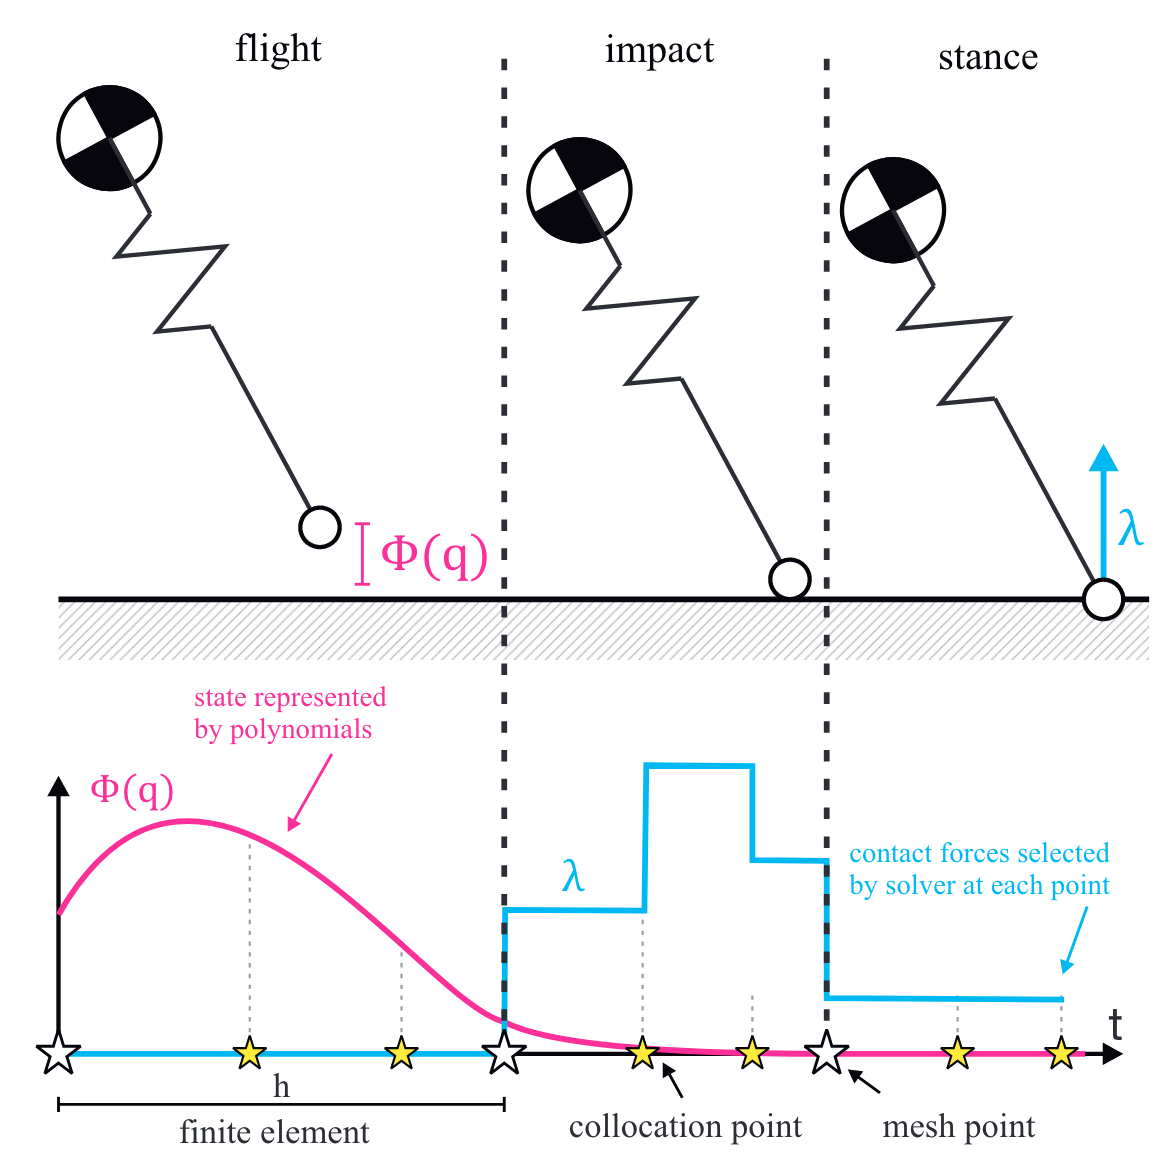
\includegraphics[width=0.4\textwidth]{figure/relaxed_method.png}}
\caption[Relaxed impact method]{Relaxed impact formulation. Contact mode is changed at each mesh point, the contact force $\lambda$ is selected by solver at each collocation point. Source: \cite{patel_contact-implicit_2019}}
\label{f_relaxed}
\end{figure}
%%%%%%%%%%%%%%%% end figure %%%%%%%%%%%%%%%%%%%

The relaxed formulation is shown in figure \ref{f_relaxed}. It implements a contact constraint that will look one time-step ahead to be able to initiate a contact force before impact. Let $C_c(\mathbf{q})$ be the relative distance between the two bodies that impact, and let the normal force $F_n$ be a control variable. The following constraints will ensure that only when the next time step is in contact ($C_c(\mathbf{q}(t+1)$) the normal force $F_n > 0$ when there is no contact at the next time step, $F_n$ must be zero:
\begin{equation}\label{e_patelimpact}
    F_n\ C_c(\mathbf{q}(t+1) = 0,\quad C_c(\mathbf{q}) \geq 0,\quad F_n \geq 0
\end{equation}
This result of this formulation is shown graphically in figure \ref{f_discontinuities}. When constraining an optimization problem likewise, the solver will find the normal forces needed to comply to the non penetration constraint $C_c(\mathbf{q}) \geq 0$. This method has been used in the optimization of an ollie. Though the initial guess needed to be similar to the solution to find feasible solutions. The model with a full body human operator took 43 minutes to solve \cite{shield_contact-implicit_2022}. 
To simplify the model I excluded this impact formulation, because I assume that the feet are always located on the skateboard, but can be out of contact by exerting zero force. In this case, where the human is not modeled with multiple segments but as a point mass, it is possible to exclude equation \ref{e_patelimpact}. By setting the normal forces of the feet $F_{p1},F_{p2}$ as control variables. The foot location is also regulated by a control variables. The acceleration is controlled instead of the foot location itself to still have smooth realistic foot trajectories. Resulting in the control variables:
\begin{equation}
    \mathbf{u}^{(1,2,3)} = [F_{p1},F_{p2},\ddot s_1, \ddot s_2]    
\end{equation}

Now that the difficult to solve contact formulation by Patel in equation \ref{e_patelimpact} is replaced by a simplified formulation, I will continue with the friction model that is used in this optimization.
Friction is present during the ollie when sliding the foot along grip-tape, when rolling, and when the tail hits the ground if the tail has a relative velocity tangential to the impact surface. Friction is a highly non-linear and discontinuous phenomenon. In general the dominant friction components that have been modeled include static friction (A force that opposes the input force at zero velocity), Coulomb friction (constant motion opposing force at non-zero velocity), viscous friction (when fluid exists between the contact surfaces), and the Stribeck effect (a speed dependent friction) \cite{makkar_new_2005}. 
\begin{figure}
    \centering
    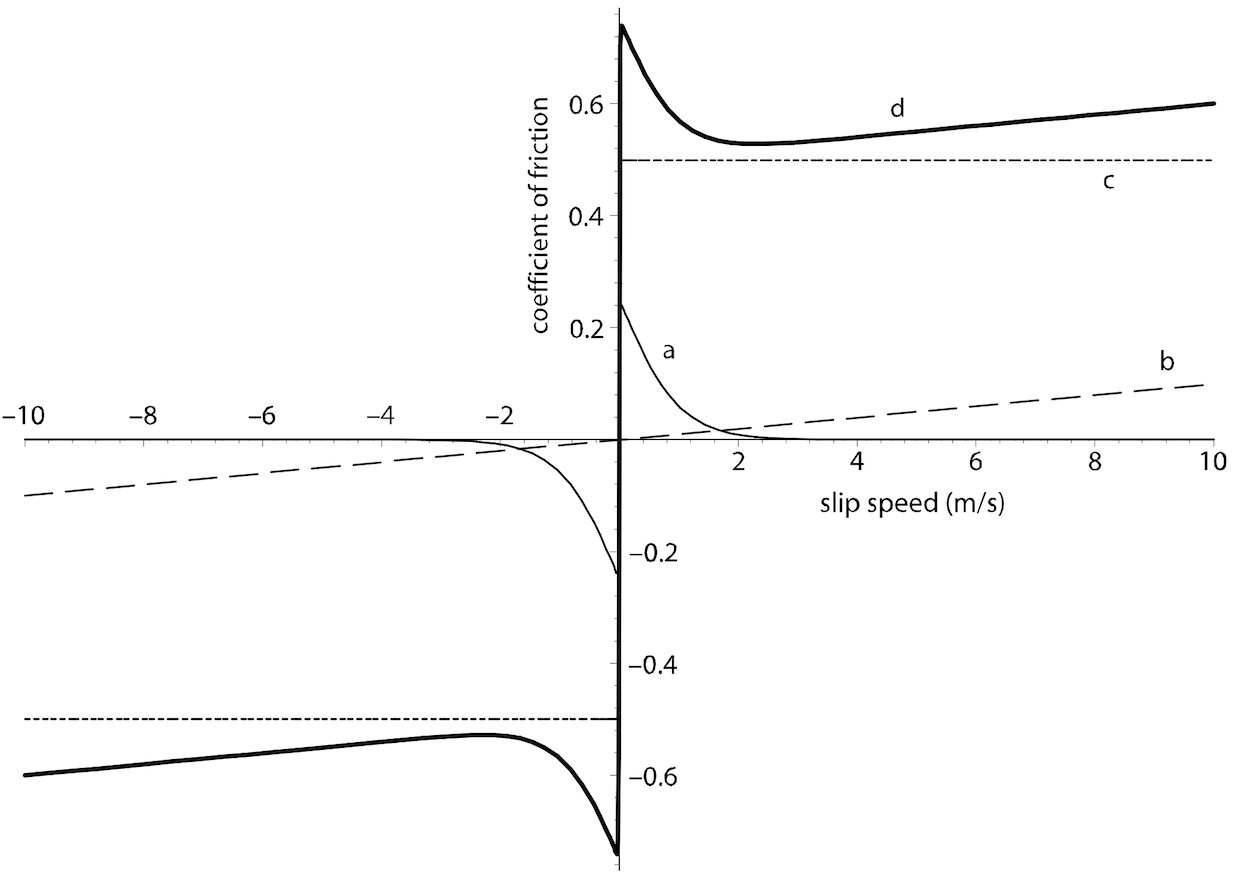
\includegraphics[width=0.4\textwidth]{figure/friction_.png}
    \caption[Friction effects]{Friction model as a composition of different effects including a) Stribeck effect, b) viscous dissipation, c) coulomb effect, d) combined model}
    \label{f_friction}
\end{figure}

%When modeling friction continuously, pure static friction does not exist since at zero velocity the friction function will be zero as well due to symmetry. 
Just like the normal force, friction can also only exist during contact. The friction is solved with a set of constraints. The first step to implement this friction is to create slack variables that divide the friction forces as described in the system dynamics $F_{f1},F_{f2}$ into a positive and negative components. For simplicity reasons I will only derive the friction of the back foot along the skateboard. The front foot friction is obtained by exactly the same process. By replacing $_1$ to $_2$ in the following equations, the front foot friction is also realized
\begin{equation} \label{e_plusminfric}
   F_{f1} = F_{f1}^+ - F_{f1}^- 
\end{equation}
As described in section \ref{s_systemdynamics}, the forces perpendicular to the skateboard are positive definite such that the force can never pull on the skateboard. Now the created slack variables also need to be positive definite:
\begin{equation}
    F_{p1} \geq 0,\quad F_{f1}^+ \geq 0,\quad F_{f1}^- \geq 0  
\end{equation}
Static and dynamic friction is bound by the friction cone shown in figure \ref{f_frictioncone}. The magnitude of dynamic friction is $F_{p1}\ \mu$ with a direction opposed to the relative sliding velocity (see figure \ref{f_frictioncone}. The static friction is bound by the whole surface of the friction cone and is only possible when the feet are not sliding. To realize this, another slack variable $\psi$ is introduced which represents the magnitude of the relative velocity $\dot s_1$ between the foot and the skateboard. 
\begin{equation}
\begin{split}
    \gamma_{18}^{(1,2,3)}: \quad & \psi_1 + \dot s_1  \geq 0 \\
    \gamma_{19}^{(1,2,3)}: \quad & \psi_1 - \dot s_1  \geq 0 \\
\end{split}
\end{equation}
Now static friction can be implemented with a set of constraints:
\begin{equation}
\begin{split}\label{e_frictioncontrol}
       \gamma_{20}^{(1,2,3)}: \quad & \mu F_{p1} - F_{f1}^+ - F_{f1}^- \geq 0 \\
       \gamma_{21}^{(1,2,3)}: \quad & (\mu F_{p1} - F_{f1}^+ - F_{f1}^-)\ \psi_1  = 0
\end{split}
\end{equation}
The first constraint assures that the positive component or the negative component of the friction is always smaller than $\mu F_{p1}$. The second constraint makes sure that when the foot slides ($\psi_1 \not = 0$),  the sum of the positive and negative friction components equal $\mu F_{p1}$. It is important that when sliding in positive direction, the negative friction component $F_{f1}^-$ should equal $\mu F_{p1}$ and $F_{f1}^+=0$ and vice versa. This is realized with the following constraints:
\begin{equation}
\begin{split}
    \gamma_{22}^{(1,2,3)}: \quad & F_{f1}^+ (\psi_1 + \dot s_1)  = 0 \\
    \gamma_{23}^{(1,2,3)}: \quad & F_{f1}^- (\psi_1 - \dot s_1)  = 0
\end{split}
\end{equation}
This type of constraint ($A\cdot B = 0$) has three possible solutions $A= 0,\ B=0,\ or\ A,B = 0$. By filling in a numerical example, the desired behaviour is shown. For example looking at the first constraint, when $\dot s_1 = -1$, then $\psi_1 + \dot s =  0$ and $F_{f1}^+$ can be a positive number. Then looking at the second constraint, when $\dot s = -1$, then $\psi - \dot s = 2$ and $F_{f1}^- = 0$. Combining this with the second equation in equation \ref{e_frictioncontrol} gives: $(\mu F_{p1} - F_{f1}^+ - 0) \cdot 0 = 0$, which results in $F_{f1}^+ = \mu F_{p1}$. This is exactly what it should be given a negative relative sliding velocity. 
The friction for the front foot will be another six constraints: $\gamma_{24-30}^{(1,2,3)}$ 
\begin{figure}
    \centering
    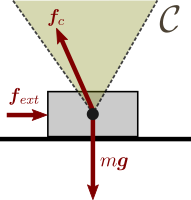
\includegraphics{figure/Frictioncone.png}
    \caption[friction cone]{$f_c$ is the reaction force exerted by the ground on the box, which is composed of a normal force $f_n$ equal and opposite to $mg$ and friction $f_w$ equal and opposite to $f_{ext}$. The box is stationary if $f_{ext} < f_n\ \mu$. Static friction is bound by $-f_n\ \mu < f_w < f_n\ \mu$. But when $f_{ext}\ >\ f_n\ \mu$, the box will start to slide with velocity $v$ and $f_w = f_n\ \mu$. Dynamic friction is described by $f_w = -sign(v) f_n\ \mu$. The top of the cone is unbound, because when a vertical external load would be applied, the normal force would change in magnitude.} 
    \footnotesize Source:\url{https://scaron.info/robot-locomotion/}
    \label{f_frictioncone}
\end{figure}

\subsubsection{Endpoint constraints} \label{p_endpoints}
\noindent To fully describe the ollie optimization problem, all phases need to be glued together. In the multi-phase optimization scheme all initial and final time variables are treated as separate variables. By constraining the corresponding variables between the phases, the variables can be treated as one variable over all three phases.

\paragraph{Impact}
\noindent Just before the skateboard is airborne, the tail hits the ground. During this collision the ground exerts a linear impulse normal to the ground. The method by Vallery and Schwab \cite{vallery_heike_advanced_2018} is based on the Newton impact law. The Newton impact law rewritten in terms of the optimization states is:
\begin{equation}\label{e_newtonimpact}
    \mathbf{\dot q_{rel}}^{(2)}(t_0) = -e\ \mathbf{\dot q_{rel}}^{(1)}(t_F)
\end{equation}
Where $\dot q_{rel}^{(2)}(t_0)$, and $\dot q_{rel}^{(1)}(t_F)$ are the relative speeds just after impact at the first collocation point of phase 2, and just before impact at the last collocation point of phase 1 respectively.  $e$, the empirical constant related to the amount of dissipated energy during impact, is called the coefficient of restitution (COR). When $e=1$ we have mechanical energy preservation, and for $e=0$ all impact energy is lost into dissipation. Now lets write this equation in matrix form. Let $C_c(\mathbf{q})$ be the relative distance normal to the contact surface. By taking the Jacobian with respect to the generalized coordinates and multiplying it with the generalized velocities we find the relative generalized velocity:
\begin{equation}\label{e_relativevelocity}
    \frac{d}{dt}\left(C_c(\mathbf{q})\right) = J_{\mathbf{q}}(C_c(\mathbf{q}))\ \mathbf{\dot q} = \mathbf{C_{c,i}}\  \mathbf{\dot q}
\end{equation}
Combine equations \ref{e_newtonimpact}, and \ref{e_relativevelocity} to get:
\begin{equation}
    \mathbf{C_{c,i}}\  \mathbf{\dot q}^{(2)}(t_0) = -e\ \mathbf{C_{c,i}}\ \mathbf{\dot q}^{(1)}(t_F)
\end{equation}
Now by introducing a Langrange multiplier $\rho_c$ which is used to solve the reaction impulse calculated with $\mathbf{C_{c,i}}\ \rho_c$ the linear impulse and momentum equation is:
\begin{equation}\label{e_linearimpulse}
    \mathbf{M_s}\ \mathbf{\dot q}^{(2)}(t_0) + \mathbf{C_{c,i}}\ \rho_c = \mathbf{M_s}\ \mathbf{\dot q}^{(1)}(t_F)
\end{equation}
Where $\mathbf{M_s}$ is the mass matrix of the system. Now writing equation \ref{e_linearimpulse} with equation \ref{e_relativevelocity} as an added constraint the velocities after impact are solved. This gives the first four endpoint constraints that define the impact of the tail:
\begin{equation}
    \beta_{1,2,3,4}: \quad \left[\begin{array}{cc}
        \mathbf{M_s} & \mathbf{C_{c,i}} \\
        \mathbf{C_{c,i}}^T & 0
    \end{array} \right]\
    \left[\begin{array}{c}
       \mathbf{\dot q}^{(2)}(t_0)  \\
        \rho_c 
    \end{array}\right] = 
    \left[\begin{array}{c}
         \mathbf{M_s}\ \mathbf{\dot q}^{(1)}(t_F)   \\
         -e\ \mathbf{C_{c,i}}^T\ \mathbf{\dot q}^{(1)}(t_F)
    \end{array}\right]
\end{equation}

Because the states in phase 1 are expressed in different variables than phase 2 as shown in section \ref{s_systemdynamics}, variables $\dot q^{(1)}(t_F)$ needs to be rewritten to the CoM coordinates $x_s,y_s$, and $\theta_s$. Also the initial values of variables $x_s^{(2)}(t_0), y_s^{(2)}(t_0)$ are dependant on the final time variables $x_w^{(1)}(t_F), \theta_s^{(1)}(t_F)$ and are set as an endpoint constraint
\footnotesize
\begin{equation}
\begin{split}
\beta_5:& \ x_s^{(2)}(t_0) = \frac{l_{w b} \cos \left(\theta_s\right)}{2}+x_w^{(1)}(t_F)-\left(-d_{c o m}+h_{t r}\right) \sin \left(\theta_s^{(1)}(t_F)\right) \\
\beta_6:& y_s^{(2)}(t_0) = \frac{l_{w b} \sin \left(\theta_s\right)}{2}+r_w+\left(-d_{c o m}+h_{t r}\right) \cos \left(\theta_s^{(1)}(t_F)\right)
\end{split}
\end{equation}
\normalsize
%%%%%%%%%%%%%%%% begin figure %%%%%%%%%%%%%%%%%%%
\begin{figure}
\centerline{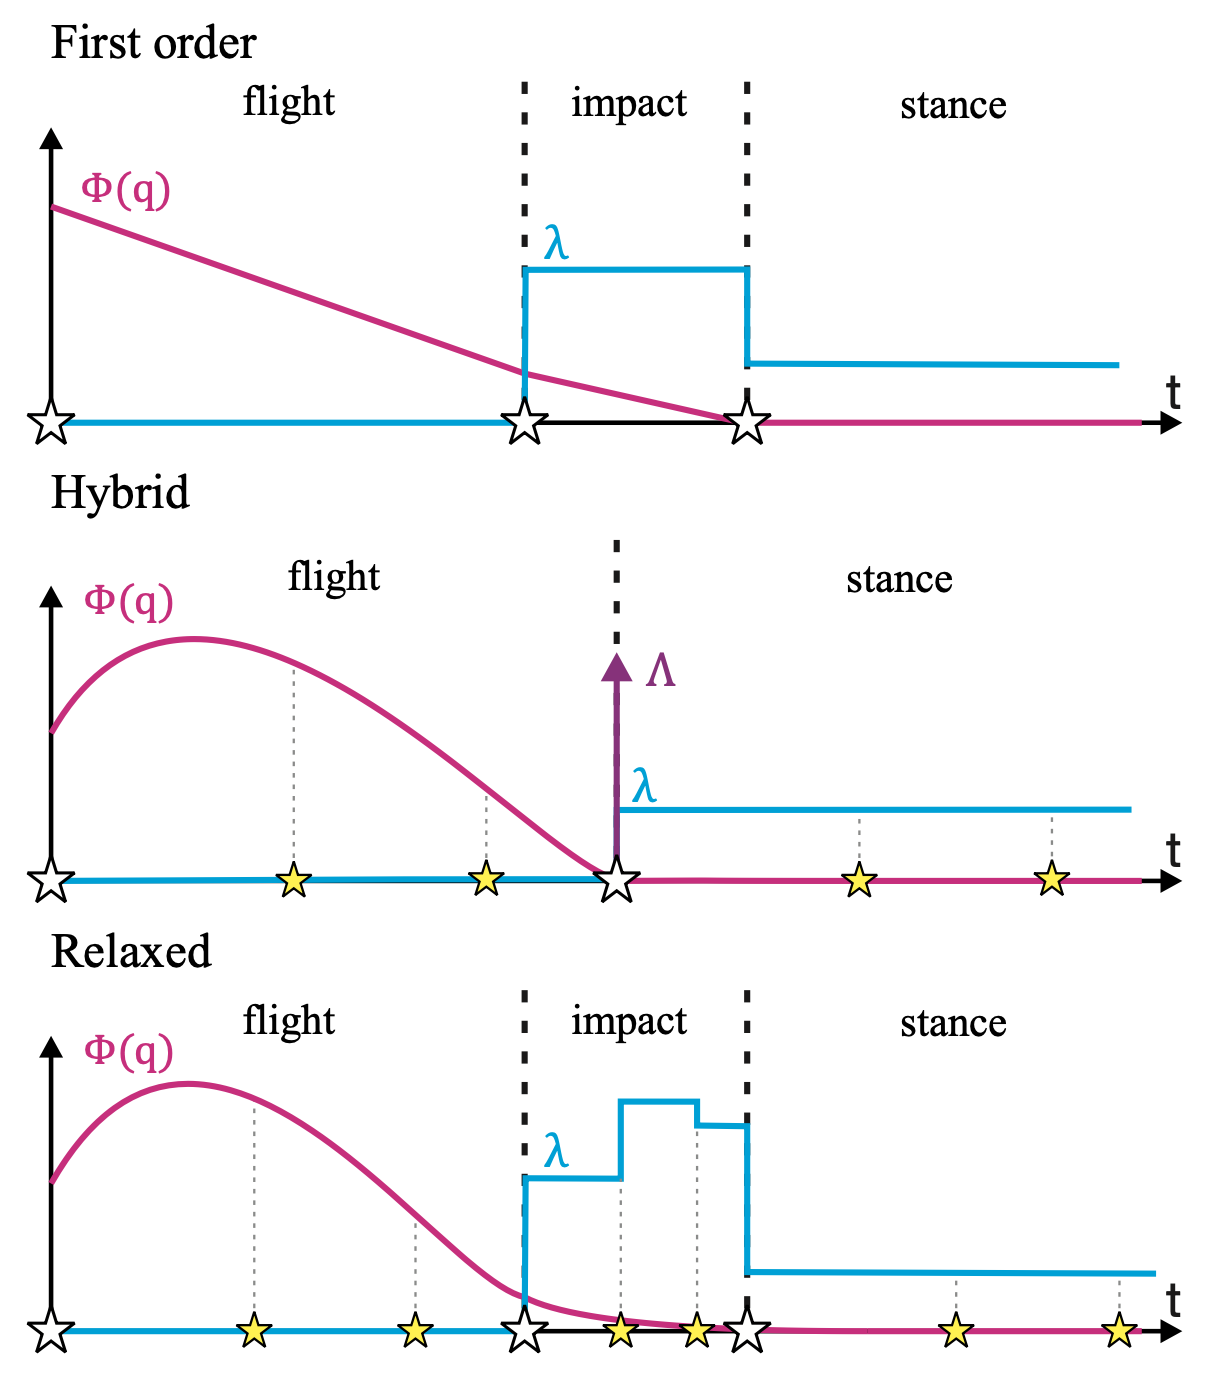
\includegraphics[width=0.3\textwidth]{figure/impactmethods.png}}
\caption{Three impact models used in optimization \cite{patel_contact-implicit_2019}. }
\label{f_discontinuities}
\end{figure}
%%%%%%%%%%%%%%%% end figure %%%%%%%%%%%%%%%%%%%

This method is a discontinuous method where velocity states will have jumps as seen in figure \ref{f_discontinuities}, second graph. This is opposed to continuous methods that will continuously change the velocity state over time (figure \ref{f_discontinuities} first graph). For example Ackerman and van den Bogert \cite{ackermann_optimality_2010} modeled the ground as a spring damper system that exerts a force when the contact point penetrates the contact surface with a gait optimization. When spring damper constants are implemented correctly, the energy should be dissipated during contact. The advantages of this model is that in an optimization the states are all continuous. This makes it possible to have unplanned impact (contact implicit optimization). In other words, you are not prescribing when and how impact occurs. The disadvantage of this model is that it is rather unaccountable for the actual force output. When solving such a problem imagine that an object is about to encounter impact and penetration depth equals 0, the states have a velocity state $v$ towards to the contact surface. The penetration depth of the next time step with a simple forward Euler integration will be $v \delta t$. This means that the magnitude of the time step will influence the penetration depth, which in terms influences the force output. The used discontinuous method will be independent of time step size and the ground does not have to be modeled complexly to get a desired force output. Furthermore, the behaviour of the impact will be constant over different iterations with different solutions, and will be more precise since a higher order optimization method can be used. 

\paragraph{Time}
\noindent The result of the optimization should be continuous in time over all three phases. This is obtained by endpoint constraints: 
\begin{equation}
    \begin{array}{c}
         \beta_7: \quad t_F^{(1)} = t_0^{(2)}  \\
         \beta_8: \quad t_F^{(2)} = t_0^{(3)}  \\
    \end{array}
\end{equation}

The time variables are set as optimization variables, meaning that the optimization should know when to switch phase. This is done by the impact angle of the skateboard. This is a function of the parameter values:
\begin{equation}
    \theta_{impact} = -\operatorname{atan}\left(\frac{h_{t r}+l_t \sin (\phi)+r_w}{-\frac{l_d}{2}-l_t \cos (\phi)+\frac{l_{w b}}{2}}\right)
\end{equation}
The end of phase 1 should equal this angle. This is obtained with endpoint constraints:
\begin{equation}
    \beta_7: \quad \theta_s^{1}(t_F) = \theta_{impact}
\end{equation}

To make sure the human starts the ollie from a standing position, the vertical forces at the beginning of phase 1 are equal to the bodyweight:
\begin{equation}
    \beta_8: \quad \mathbf{F_h} \cdot \mathbf{\hat n_y} = m_h g
\end{equation}

The definition of landing the ollie has been set to the back wheel touching the ground at a minimum of 0 [rad] (level) and a maximum of $\frac{1}{6} \pi$[rad] (rotated counter clockwise sligthly). The optimization stops when the backwheel touches the ground.

\begin{equation}
    \beta_9 : \frac{-l_{wb}}{2} \sin(\theta_s(t_F^{(2)})) - r_w + y_s(t_F^{(2)}) + (d_{com} - {d_tr}) \cos(\theta_s(t_F^{(2)}))
\end{equation}
Variables $\theta_s, s_1, s_2, \dot s_1, \dot s_2, x_h, y_h, \dot x_h, \dot y_h$ have equal endpoints between phase 1 and 2 ($b_{9-18})$. All state variables have equal endpoints between phase 2 and 3 ($b_{18-32}$). Initial and final endpoint constraints are set to a wide range and are found in Appendix B, \ref{t_constraints}.
